
%%%%%%%%%%%%%%%%%%%%%%%%%%%%%%%%%%%%%%%%%%%%%%%%%%%%%%%%%%%%%%%%%%%%%%%%%%%%%%
% Copyright (c) 2003-2016 by The University of Queensland
% http://www.uq.edu.au
%
% Primary Business: Queensland, Australia
% Licensed under the Open Software License version 3.0
% http://www.opensource.org/licenses/osl-3.0.php
%
% Development until 2012 by Earth Systems Science Computational Center (ESSCC)
% Development 2012-2013 by School of Earth Sciences
% Development from 2014 by Centre for Geoscience Computing (GeoComp)
%
%%%%%%%%%%%%%%%%%%%%%%%%%%%%%%%%%%%%%%%%%%%%%%%%%%%%%%%%%%%%%%%%%%%%%%%%%%%%%%

\section{The First Steps}\label{FirstSteps} 
In this chapter we give an introduction how to use \escript to solve 
a partial differential equation\index{partial differential equation} (PDE\index{partial differential equation!PDE}).
We assume you are at least a little familiar with \PYTHON.
The knowledge presented in the \PYTHON tutorial at \url{https://docs.python.org/2/tutorial/} is more than sufficient.

The PDE\index{partial differential equation} we wish to solve is the Poisson equation\index{Poisson equation} 
\begin{equation}
    -\Delta u=f 
    \label{eq:FirstSteps.1}
\end{equation}
for the solution $u$. The function $f$ is the given right hand side. The domain of interest, denoted by $\Omega$,
is the unit square 
\begin{equation}
\Omega=[0,1]^2=\{ (x_0;x_1) | 0\le x_{0} \le 1 \mbox{ and } 0\le x_{1} \le 1 \}
\label{eq:FirstSteps.1b}
\end{equation}
The domain is shown in \fig{fig:FirstSteps.1}.
\begin{figure}[ht]
    \centerline{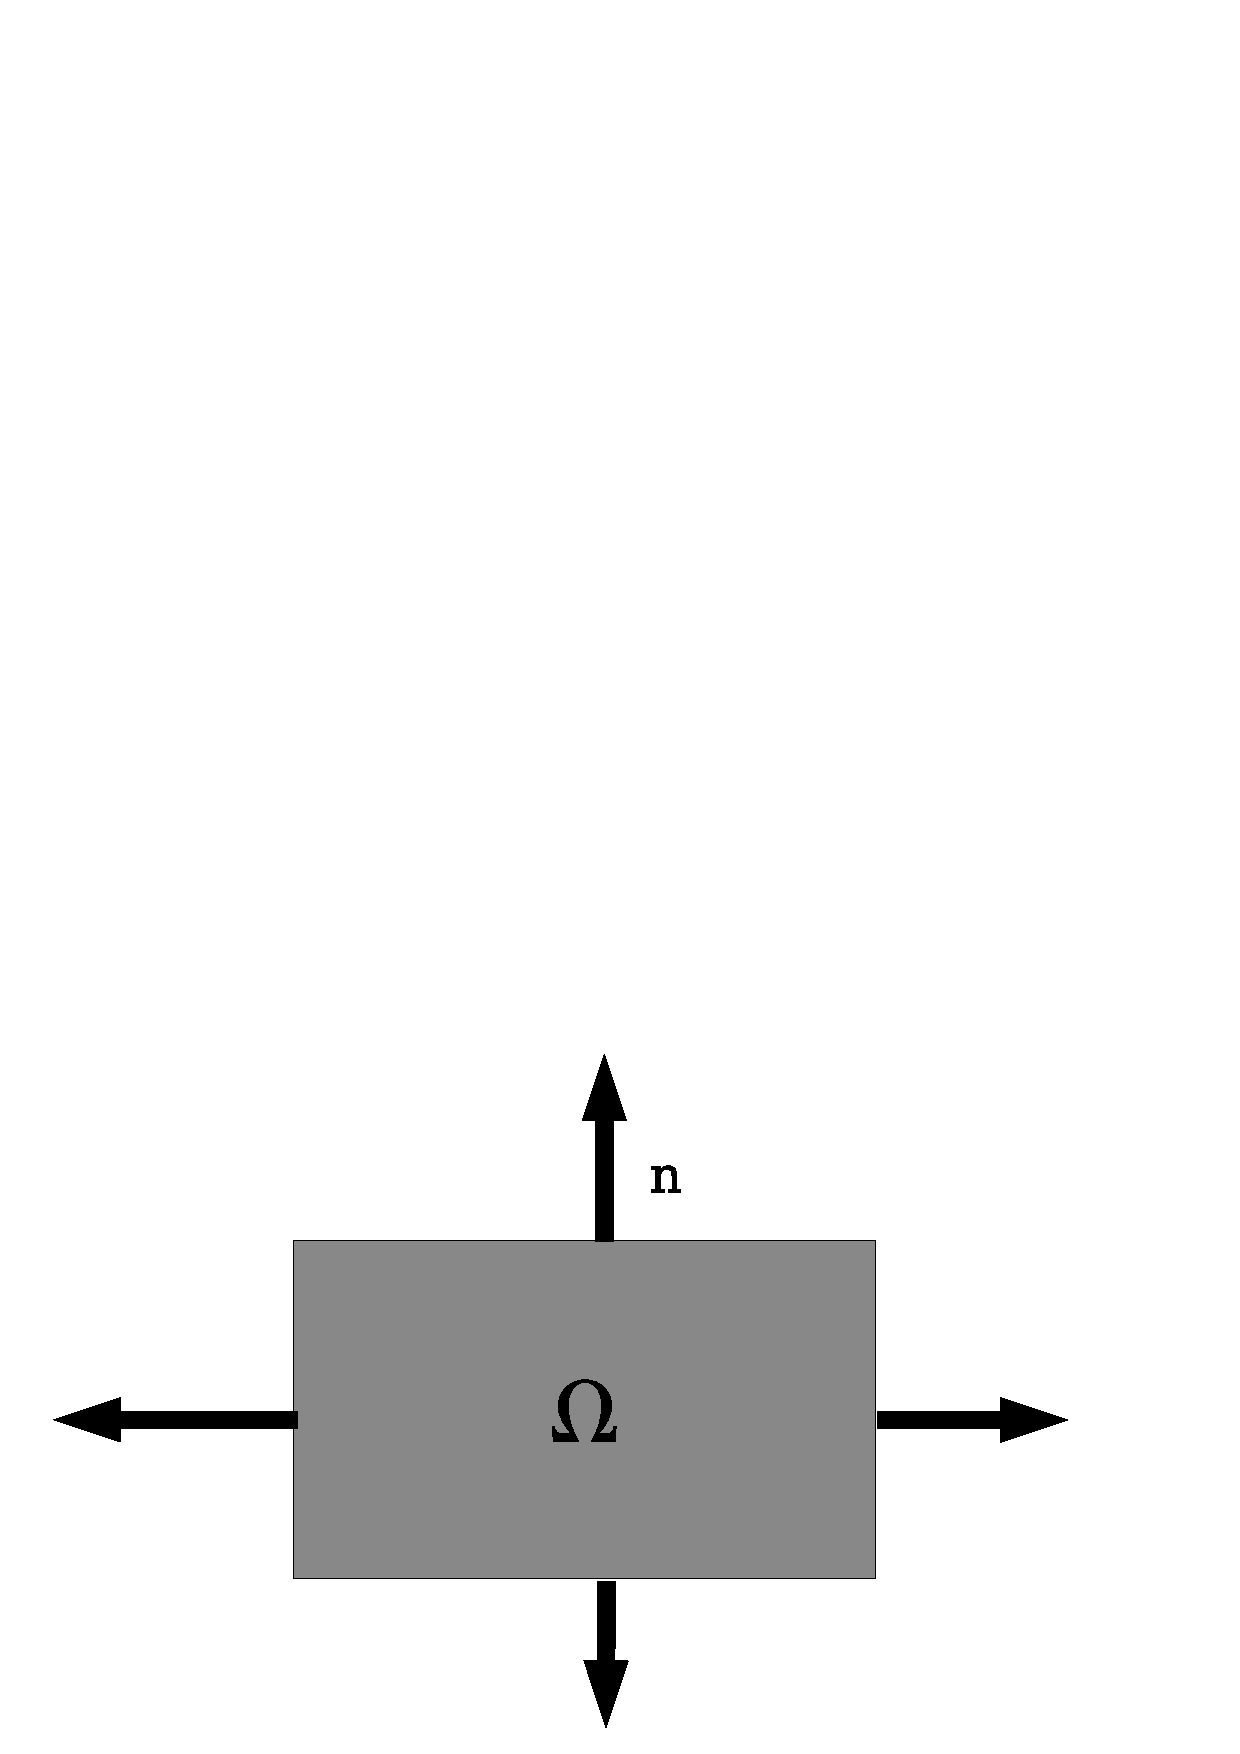
\includegraphics{FirstStepDomain}}
    \caption{Domain $\Omega=[0,1]^2$ with outer normal field $n$.}
    \label{fig:FirstSteps.1}
\end{figure}

$\Delta$ denotes the Laplace operator\index{Laplace operator}, which is defined by
\begin{equation}
\Delta u = (u_{,0})_{,0}+(u_{,1})_{,1}
\label{eq:FirstSteps.1.1}
\end{equation}
where, for any function $u$ and any direction $i$, $u_{,i}$
denotes the partial derivative \index{partial derivative} of $u$ with respect
to $i$.\footnote{You may be more familiar with the Laplace
operator\index{Laplace operator} being written as $\nabla^2$, and written in
the form
\begin{equation*}
    \nabla^2 u = \nabla^t \cdot \nabla u =  \frac{\partial^2 u}{\partial x_0^2} 
    + \frac{\partial^2 u}{\partial  x_1^2}
\end{equation*}
and \eqn{eq:FirstSteps.1} as
\begin{equation*}
    -\nabla^2 u = f
\end{equation*}
}
Basically, in the subindex of a function, any index to the right of the comma denotes a spatial derivative with respect 
to the index. To get a more compact form we will write $u_{,ij}=(u_{,i})_{,j}$
which leads to
\begin{equation}
\Delta u = u_{,00}+u_{,11}=\sum_{i=0}^2 u_{,ii}
\label{eq:FirstSteps.1.1b}
\end{equation}
We often find that use
of nested $\sum$ symbols makes formulas cumbersome, and we use the more
compact Einstein summation convention\index{summation convention}. This 
drops the $\sum$ sign and assumes that a summation is performed over any repeated index.
For instance we write
\begin{eqnarray}
x_{i}y_{i}=\sum_{i=0}^2 x_{i}y_{i}   \\
x_{i}u_{,i}=\sum_{i=0}^2 x_{i}u_{,i}   \\
u_{,ii}=\sum_{i=0}^2 u_{,ii} \\
x_{ij}u_{i,j}=\sum_{j=0}^2\sum_{i=0}^2 x_{ij}u_{i,j}   \\
\label{eq:FirstSteps.1.1c}
\end{eqnarray}
With the summation convention we can write the Poisson equation \index{Poisson equation} as
\begin{equation}
- u_{,ii} =1 
\label{eq:FirstSteps.1.sum}
\end{equation}
where $f=1$ in this example.

On the boundary of the domain $\Omega$ the normal derivative $n_{i} u_{,i}$
of the solution $u$ shall be zero, i.e. $u$ shall fulfill
the homogeneous Neumann boundary condition\index{Neumann
boundary condition!homogeneous}
\begin{equation}
n_{i} u_{,i}= 0 \;.
\label{eq:FirstSteps.2}
\end{equation}
$n=(n_{i})$ denotes the outer normal field
of the domain, see \fig{fig:FirstSteps.1}. Remember that we 
are applying the Einstein summation convention \index{summation convention}, i.e. $n_{i} u_{,i}= n_{0} u_{,0} +%
n_{1} u_{,1}$.\footnote{Some readers may familiar with the
notation $\frac{\partial u}{\partial n} = n_{i} u_{,i}$
for the normal derivative.}
The Neumann boundary condition of \eqn{eq:FirstSteps.2} should be fulfilled on the
set $\Gamma^N$ which is the top and right edge of the domain:
\begin{equation}
    \Gamma^N=\{(x_0;x_1) \in \Omega | x_{0}=1 \mbox{ or } x_{1}=1  \}
    \label{eq:FirstSteps.2b}
\end{equation}
On the bottom and the left edge of the domain which is defined
as 
\begin{equation}
    \Gamma^D=\{(x_0;x_1) \in \Omega | x_{0}=0 \mbox{ or } x_{1}=0  \}
    \label{eq:FirstSteps.2c}
\end{equation}
the solution shall be identical to zero:
\begin{equation}
    u=0 \; .
    \label{eq:FirstSteps.2d}
\end{equation}
This kind of boundary condition is called a homogeneous Dirichlet boundary
condition\index{Dirichlet boundary condition!homogeneous}.
The partial differential equation in \eqn{eq:FirstSteps.1.sum} together
with the Neumann boundary condition \eqn{eq:FirstSteps.2} and 
Dirichlet boundary condition in \eqn{eq:FirstSteps.2d} form a so-called
boundary value
problem\index{boundary value problem} (BVP\index{boundary value problem!BVP})
for the unknown function~$u$. 

\begin{figure}[ht]
    \centerline{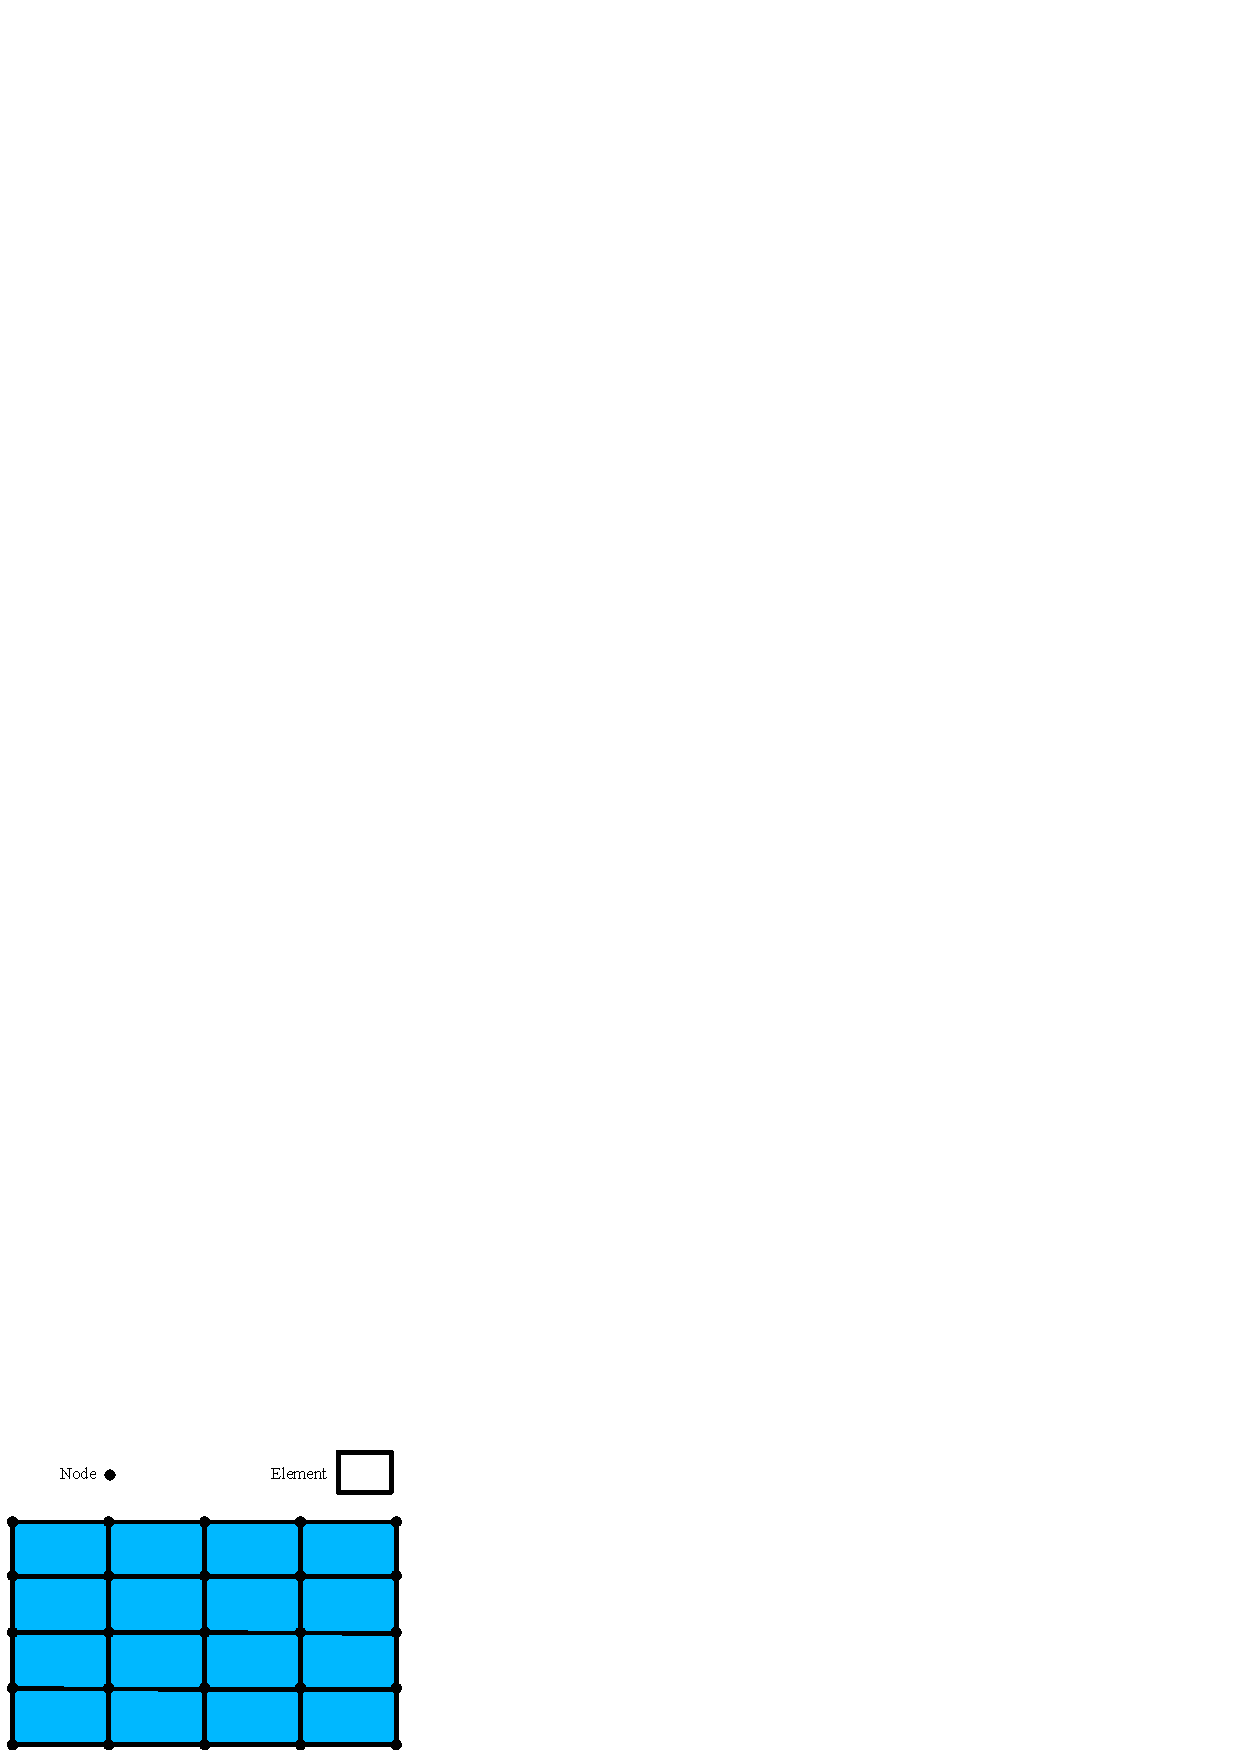
\includegraphics{FirstStepMesh}}
    \caption{Mesh of $4 \times 4$ elements on a rectangular domain. Here
    each element is a quadrilateral and described by four nodes, namely
    the corner points. The solution is interpolated by a bi-linear
    polynomial.}
    \label{fig:FirstSteps.2}
\end{figure}

In general the BVP\index{boundary value problem!BVP} cannot be solved
analytically and numerical methods have to be used to construct an
approximation of the solution $u$.
Here we will use the finite element method\index{finite element method}
(FEM\index{finite element method!FEM}).
The basic idea is to fill the domain with a set of points called nodes.
The solution is approximated by its values on the nodes\index{finite element method!nodes}.
Moreover, the domain is subdivided into smaller sub-domains called
elements\index{finite element method!element}.
On each element the solution is represented by a polynomial of a certain
degree through its values at the nodes located in the element.
The nodes and their connection through elements is called a
mesh\index{finite element method!mesh}. \fig{fig:FirstSteps.2} shows an
example of a FEM mesh with four elements in the $x_0$ and four elements
in the $x_1$ direction over the unit square.
For more details we refer the reader to the literature, for instance \Ref{Zienc,NumHand}.

The \escript solver we want to use to solve this problem is embedded into the \PYTHON interpreter language.
So you can solve the problem interactively but you will learn quickly that it
is more efficient to use scripts which you can edit with your favorite editor.
To enter the escript environment, use the \program{run-escript}
command\footnote{\program{run-escript} is not available under Windows.
If you run under Windows you can just use the \program{python} command and the
\env{OMP_NUM_THREADS} environment variable to control the number of threads.}:
\begin{verbatim}
run-escript
\end{verbatim}
which will pass you on to the \PYTHON prompt
\begin{verbatim}
Python 2.7.6 (default, Mar 22 2014, 15:40:47) 
[GCC 4.8.2] on linux2
Type "help", "copyright", "credits" or "license" for more information.
>>> 
\end{verbatim}
Here you can use all available \PYTHON commands and language features\footnote{Throughout our examples, we use the python 3 form of 
print. That is, print(1) instead of print 1.}, for instance
\begin{python}
  >>> x=2+3
  >>> print("2+3=",x)
  2+3= 5
\end{python}
We refer to the \PYTHON user's guide if you are not familiar with \PYTHON.

\escript provides the class \Poisson to define a Poisson equation\index{Poisson equation}.
(We will discuss a more general form of a PDE\index{partial differential equation!PDE} 
that can be defined through the \LinearPDE class later.)
The instantiation of a \Poisson class object requires the specification of the domain $\Omega$.
In \escript the \Domain class objects are used to describe the geometry of a
domain but it also contains information about the discretization methods and
the actual solver which is used to solve the PDE.
Here we are using the FEM\index{finite element method} library \finley.
The following statements create the \Domain object \var{mydomain} from the 
\finley function \method{Rectangle}:
\begin{python}
  from esys.finley import Rectangle
  mydomain = Rectangle(l0=1.,l1=1.,n0=40, n1=20)
\end{python}
In this case the domain is a rectangle with the lower left corner at point $(0,0)$
and the upper right corner at $(\var{l0},\var{l1})=(1,1)$.
The arguments \var{n0} and \var{n1} define the number of elements in $x_{0}$ and
$x_{1}$-direction respectively. For more details on \method{Rectangle} and
other \Domain generators see \Chap{chap:finley}, \Chap{chap:ripley}, and
\Chap{chap:speckley}.

The following statements define the \Poisson class object \var{mypde} with domain \var{mydomain} and
the right hand side $f$ of the PDE to constant $1$: 
\begin{python}
  from esys.escript.linearPDEs import Poisson
  mypde = Poisson(mydomain)
  mypde.setValue(f=1)
\end{python}
We have not specified any boundary condition but the \Poisson class implicitly
assumes homogeneous Neuman boundary conditions\index{Neumann boundary condition!homogeneous} defined by \eqn{eq:FirstSteps.2}.
With this boundary condition the BVP\index{boundary value problem!BVP} we have
defined has no unique solution.
In fact, with any solution $u$ and any constant $C$ the function $u+C$ becomes
a solution as well.
We have to add a Dirichlet boundary condition\index{Dirichlet boundary condition}.
This is done by defining a characteristic function\index{characteristic function}
which has positive values at locations $x=(x_{0},x_{1})$
where Dirichlet boundary condition is set and $0$ elsewhere.
In our case of $\Gamma^D$ defined by \eqn{eq:FirstSteps.2c}, we need to
construct a function \var{gammaD} which is positive for the cases $x_{0}=0$ or $x_{1}=0$.
To get an object \var{x} which contains the coordinates of the nodes in the domain use
\begin{python}
  x=mydomain.getX() 
\end{python}
The method \method{getX} of the \Domain \var{mydomain} gives access to locations
in the domain defined by \var{mydomain}.
The object \var{x} is actually a \Data object which will be discussed in
\Chap{ESCRIPT CHAP} in more detail.
What we need to know here is that \var{x} has \Rank (number of dimensions) and
a \Shape (list of dimensions) which can be viewed by calling the \method{getRank} and \method{getShape} methods:
\begin{python}
  print("rank ",x.getRank(),", shape ",x.getShape())
\end{python}
This will print something like
\begin{python}
  rank 1, shape (2,)
\end{python}
The \Data object also maintains type information which is represented by the 
\FunctionSpace of the object. For instance
\begin{python}
  print(x.getFunctionSpace())
\end{python}
will print 
\begin{python}
  Finley_Nodes [ContinuousFunction(domain)] on FinleyMesh 
\end{python}
which tells us that the coordinates are stored on the nodes of (rather than on
points in the interior of) a Finley mesh.
To get the  $x_{0}$ coordinates of the locations we use the statement 
\begin{python}
  x0=x[0]
\end{python}
Object \var{x0} is again a \Data object now with \Rank $0$ and \Shape $()$.
It inherits the \FunctionSpace from \var{x}:
\begin{python}
  print(x0.getRank(), x0.getShape(), x0.getFunctionSpace())
\end{python}
will print
\begin{python}
  0 () Finley_Nodes [ContinuousFunction(domain)] on FinleyMesh
\end{python}
We can now construct a function \var{gammaD} which is only non-zero on the
bottom and left edges of the domain with
\begin{python}
  from esys.escript import whereZero
  gammaD=whereZero(x[0])+whereZero(x[1])
\end{python}

\code{whereZero(x[0])} creates a function which equals $1$ where \code{x[0]} is (almost) equal to zero and $0$ elsewhere. 
Similarly, \code{whereZero(x[1])} creates a function which equals $1$ where \code{x[1]} is equal to zero and $0$ elsewhere.
The sum of the results of \code{whereZero(x[0])} and \code{whereZero(x[1])}
gives a function on the domain \var{mydomain} which is strictly positive where $x_{0}$ or $x_{1}$ is equal to zero.
Note that \var{gammaD} has the same \Rank, \Shape and \FunctionSpace like \var{x0} used to define it.
So from 
\begin{python}
  print(gammaD.getRank(), gammaD.getShape(), gammaD.getFunctionSpace())
\end{python}
one gets 
\begin{python}
  0 () Finley_Nodes [ContinuousFunction(domain)] on FinleyMesh
\end{python}
An additional parameter \var{q} of the \code{setValue} method of the \Poisson
class defines the characteristic function\index{characteristic function} of
the locations of the domain where the homogeneous Dirichlet boundary condition\index{Dirichlet boundary condition!homogeneous} is set.
The complete definition of our example is now:
\begin{python}
  from esys.escript.linearPDEs import Poisson
  x = mydomain.getX()
  gammaD = whereZero(x[0])+whereZero(x[1])
  mypde = Poisson(domain=mydomain)
  mypde.setValue(f=1,q=gammaD)
\end{python}
The first statement imports the \Poisson class definition from the \linearPDEs module.
To get the solution of the Poisson equation defined by \var{mypde} we just have to call its \method{getSolution} method. 

Now we can write the script to solve our Poisson problem
\begin{python}
  from esys.escript import *
  from esys.escript.linearPDEs import Poisson
  from esys.finley import Rectangle
  # generate domain:
  mydomain = Rectangle(l0=1.,l1=1.,n0=40, n1=20)
  # define characteristic function of Gamma^D
  x = mydomain.getX()
  gammaD = whereZero(x[0])+whereZero(x[1])
  # define PDE and get its solution u
  mypde = Poisson(domain=mydomain)
  mypde.setValue(f=1, q=gammaD)
  u = mypde.getSolution()
\end{python}
The question is what we do with the calculated solution \var{u}.
Besides postprocessing, e.g. calculating the gradient or the average value,
which will be discussed later, plotting the solution is one of the things you
might want to do.
\escript offers two ways to do this, both based on external modules or packages.
The first option is using the \MATPLOTLIB module which allows plotting 2D
results relatively quickly from within the \PYTHON script, see~\cite{matplotlib}.
However, there are limitations when using this tool, especially for large
problems and when solving three-dimensional problems.
Therefore, \escript provides functionality to export data as files which can
subsequently be read by third-party software packages such as
\mayavi\cite{mayavi} or \VisIt~\cite{VisIt}.

\subsection{Plotting Using \MATPLOTLIB}
The \MATPLOTLIB module provides a simple and easy-to-use way to visualize PDE
solutions (or other \Data objects).
To hand over data from \escript to \MATPLOTLIB the values need to be mapped onto
a rectangular grid. We will make use of the \numpy module for this.

First we need to create a rectangular grid which is accomplished by the following statements:
\begin{python}
  import numpy
  x_grid = numpy.linspace(0., 1., 50)
  y_grid = numpy.linspace(0., 1., 50)
\end{python}
\var{x_grid} is an array defining the x coordinates of the grid while
\var{y_grid} defines the y coordinates of the grid.
In this case we use $50$ points over the interval $[0,1]$ in both directions. 

Now the values created by \escript need to be interpolated to this grid.
We will use the \MATPLOTLIB \function{mlab.griddata} function to do this.
Spatial coordinates are easily extracted as a \var{list} by
\begin{python}
  x=mydomain.getX()[0].toListOfTuples()
  y=mydomain.getX()[1].toListOfTuples()
\end{python}
In principle we can apply the same \member{toListOfTuples} method to extract the values from the PDE solution \var{u}.
However, we have to make sure that the \Data object we extract the values from
uses the same \FunctionSpace as we have used when extracting \var{x} and \var{y}.
We apply the \function{interpolation} to \var{u} before extraction to achieve this:
\begin{python}
  z=interpolate(u, mydomain.getX().getFunctionSpace())
\end{python}
The values in \var{z} are the values at the points with the coordinates given by \var{x} and \var{y}.
These values are interpolated to the grid defined by \var{x_grid} and \var{y_grid} by using
\begin{python}
  import matplotlib
  z_grid = matplotlib.mlab.griddata(x, y, z, xi=x_grid, yi=y_grid)
\end{python}
Now \var{z_grid} gives the values of the PDE solution \var{u} at the grid which can be plotted using \function{contourf}:
\begin{python}
  matplotlib.pyplot.contourf(x_grid, y_grid, z_grid, 5)
  matplotlib.pyplot.savefig("u.png")
\end{python}
Here we use 5 contours. The last statement writes the plot to the file \file{u.png} in the PNG format.
Alternatively, one can use 
\begin{python}
  matplotlib.pyplot.contourf(x_grid, y_grid, z_grid, 5)
  matplotlib.pyplot.show()
\end{python}
which gives an interactive browser window.

\begin{figure}
\centerline{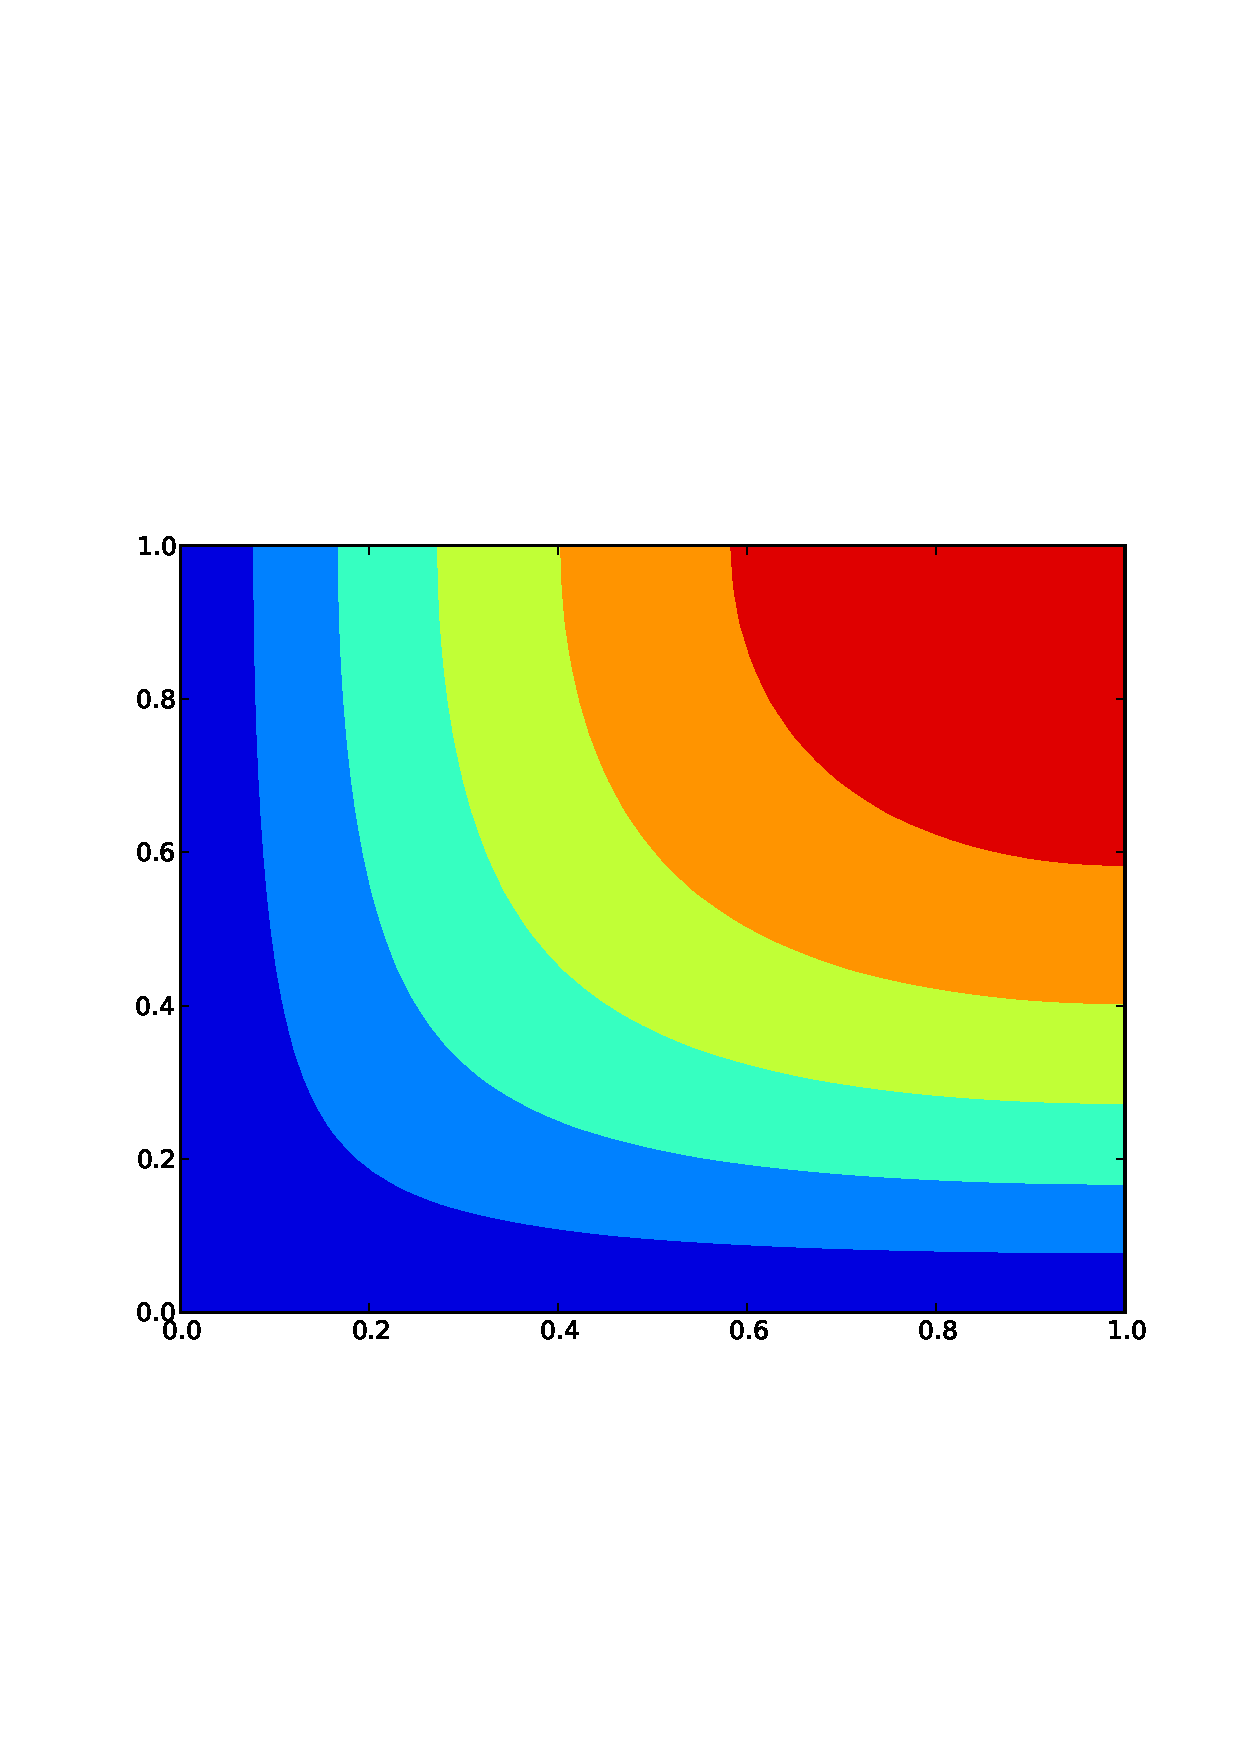
\includegraphics[width=\figwidth]{FirstStepResultMATPLOTLIB}}
\caption{Visualization of the Poisson Equation Solution for $f=1$ using \MATPLOTLIB}
\label{fig:FirstSteps.3b}
\end{figure}

Now we can write the script to solve our Poisson problem
\begin{python}
  from esys.escript import *
  from esys.escript.linearPDEs import Poisson
  from esys.finley import Rectangle
  import numpy
  import matplotlib
  import pylab
  # generate domain:
  mydomain = Rectangle(l0=1.,l1=1.,n0=40, n1=20)
  # define characteristic function of Gamma^D
  x = mydomain.getX()
  gammaD = whereZero(x[0])+whereZero(x[1])
  # define PDE and get its solution u
  mypde = Poisson(domain=mydomain)
  mypde.setValue(f=1,q=gammaD)
  u = mypde.getSolution()
  # interpolate u to a matplotlib grid:
  x_grid = numpy.linspace(0.,1.,50)
  y_grid = numpy.linspace(0.,1.,50)
  x=mydomain.getX()[0].toListOfTuples()
  y=mydomain.getX()[1].toListOfTuples()
  z=interpolate(u,mydomain.getX().getFunctionSpace()).toListOfTuples()
  z_grid = matplotlib.mlab.griddata(x,y,z,xi=x_grid,yi=y_grid )
  # interpolate u to a rectangular grid:
  matplotlib.pyplot.contourf(x_grid, y_grid, z_grid, 5)
  matplotlib.pyplot.savefig("u.png")
\end{python}
The entire code is available as \file{poisson_matplotlib.py} in the \ExampleDirectory.
You can run the script using the {\it escript} environment
\begin{verbatim}
run-escript poisson_matplotlib.py
\end{verbatim}
This will create a file called \file{u.png}, see \fig{fig:FirstSteps.3b}.
For details on the usage of the \MATPLOTLIB module we refer to the documentation~\cite{matplotlib}.

As pointed out, \MATPLOTLIB is restricted to the two-dimensional case and
should be used for small problems only.
It can not be used under \MPI as the \member{toListOfTuples} method is not
safe under \MPI\footnote{The phrase 'safe under \MPI' means that a program
will produce correct results when run on more than one processor under \MPI.}.

\begin{figure}
\centerline{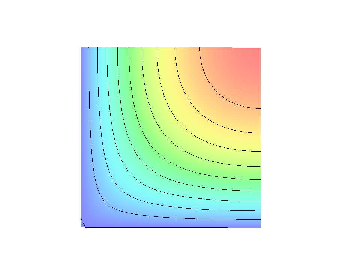
\includegraphics[width=\figwidth]{FirstStepResult}}
\caption{Visualization of the Poisson Equation Solution for $f=1$}
\label{fig:FirstSteps.3}
\end{figure}

\subsection{Visualization using export files}

As an alternative to \MATPLOTLIB, {\it escript} supports exporting data to
\VTK and \SILO files which can be read by visualization tools such as
\mayavi\cite{mayavi} and \VisIt~\cite{VisIt}. This method is \MPI safe and
works with large 2D and 3D problems.

To write the solution \var{u} of the Poisson problem in the \VTK file format
to the file \file{u.vtu} one needs to add:
\begin{python}
  from esys.weipa import saveVTK
  saveVTK("u.vtu", sol=u)
\end{python}
This file can then be opened in a \VTK compatible visualization tool where the
solution is accessible by the name {\it sol}. Similarly,
\begin{python}
  from esys.weipa import saveSilo
  saveSilo("u.silo", sol=u)
\end{python}
will write \var{u} to a \SILO file if escript was compiled with support for
LLNL's \SILO library.

The Poisson problem script is now 
\begin{python}
  from esys.escript import *
  from esys.escript.linearPDEs import Poisson
  from esys.finley import Rectangle
  from esys.weipa import saveVTK
  # generate domain:
  mydomain = Rectangle(l0=1.,l1=1.,n0=40, n1=20)
  # define characteristic function of Gamma^D
  x = mydomain.getX()
  gammaD = whereZero(x[0])+whereZero(x[1])
  # define PDE and get its solution u
  mypde = Poisson(domain=mydomain)
  mypde.setValue(f=1,q=gammaD)
  u = mypde.getSolution()
  # write u to an external file
  saveVTK("u.vtu",sol=u)
\end{python}
The entire code is available as \file{poisson_vtk.py} in the \ExampleDirectory.

You can run the script using the {\it escript} environment and visualize the
solution using \mayavi:
\begin{verbatim}
run-escript poisson_vtk.py
mayavi2 -d u.vtu -m Surface
\end{verbatim}
The result is shown in \fig{fig:FirstSteps.3}.

